%===================================================================================
% JORNADA CIENTÍFICA ESTUDIANTIL - MATCOM, UH
%===================================================================================
% Esta plantilla ha sido diseñada para ser usada en los artículos de la
% Jornada Científica Estudiantil, MatCom.
%
% Por favor, siga las instrucciones de esta plantilla y rellene en las secciones
% correspondientes.
%
% NOTA: Necesitará el archivo 'jcematcom.sty' en la misma carpeta donde esté este
%       archivo para poder utilizar esta plantila.
%===================================================================================



%===================================================================================
% PREÁMBULO
%-----------------------------------------------------------------------------------
\documentclass[a4paper,10pt,twocolumn]{report}

%===================================================================================
% Paquetes
%-----------------------------------------------------------------------------------
\usepackage{amsmath}
\usepackage{amsfonts}
\usepackage{amssymb}
\usepackage{jcematcom}
\usepackage[utf8]{inputenc}
\usepackage{listings}
\usepackage[pdftex]{hyperref}
\usepackage{float}
%-----------------------------------------------------------------------------------
% Configuración
%-----------------------------------------------------------------------------------
\hypersetup{colorlinks,%
	    citecolor=black,%
	    filecolor=black,%
	    linkcolor=black,%
	    urlcolor=blue}

\lstset{ %
	language=R, % lenguaje
	basicstyle=\footnotesize\ttfamily,
	tabsize=2,
	stringstyle=\ttfamily,
	keywordstyle=\color{blue},
	commentstyle=\color{brown}
	showstringspaces=false
}
			
%===================================================================================



%===================================================================================
% Presentacion
%-----------------------------------------------------------------------------------
% Título
%-----------------------------------------------------------------------------------
\title{Proyecto de Estadística Primera Fase - Household}

%-----------------------------------------------------------------------------------
% Autores
%-----------------------------------------------------------------------------------
\author{\\
\name Loraine Monteagudo García \email \href{mailto:l.monteagudo@estudiantes.matcom.uh.cu}{l.monteagudo@estudiantes.matcom.uh.cu}
	\\ \addr Grupo C411 \AND
\name Amanda Marrero Santos \email \href{mailto:a.marrero@estudiantes.matcom.uh.cu}{a.marrero@estudiantes.matcom.uh.cu}
  \\ \addr Grupo C411 \AND
  \name Manuel S. Fernández Arias \email \href{mailto:m.fernandez2@estudiantes.matcom.uh.cu}{m.fernandez2@estudiantes.matcom.uh.cu}
	\\ \addr Grupo C411}

%-----------------------------------------------------------------------------------
% Tutores
%-----------------------------------------------------------------------------------
\tutors{\\
Lic. Dalia Díaz Sistach, \emph{Universidad de la Habana, Facultad de Matemática y Computación}}

%-----------------------------------------------------------------------------------
% Headings
%-----------------------------------------------------------------------------------
\jcematcomheading{\the\year}{1-\pageref{end}}{Loraine Monteagudo, Amanda Marrero, Manuel Fernández}

%-----------------------------------------------------------------------------------
\ShortHeadings{Household}{Autores}
%===================================================================================



%===================================================================================
% DOCUMENTO
%-----------------------------------------------------------------------------------
\begin{document}

%-----------------------------------------------------------------------------------
% NO BORRAR ESTA LINEA!
%-----------------------------------------------------------------------------------
\twocolumn[
%-----------------------------------------------------------------------------------

\maketitle

%===================================================================================
% Resumen y Abstract
%-----------------------------------------------------------------------------------
\selectlanguage{spanish} % Para producir el documento en Español

%-----------------------------------------------------------------------------------
% Resumen en Español
%-----------------------------------------------------------------------------------
% \begin{abstract}

% 	El Resumen en Español debe constar de $100$ a $200$ palabras y presentar de forma
% 	clara y concisa el contenido fundamental del artículo.

% \end{abstract}

%-----------------------------------------------------------------------------------
% English Abstract
%-----------------------------------------------------------------------------------
\vspace{0.5cm}

% \begin{enabstract}

%   The English Abstract must have have $100$ to $200$ words, and present in a clear
%   and concise form the essentials of the article content.

% \end{enabstract}

%-----------------------------------------------------------------------------------
% Palabras clave
%-----------------------------------------------------------------------------------
% \begin{keywords}
% 	Separadas,
% 	Por,
% 	Comas.
% \end{keywords}

%-----------------------------------------------------------------------------------
% Temas
%-----------------------------------------------------------------------------------
% \begin{topics}
% 	Tema, Subtema.
% \end{topics}


%-----------------------------------------------------------------------------------
% NO BORRAR ESTAS LINEAS!
%-----------------------------------------------------------------------------------
\vspace{0.8cm}
]
%-----------------------------------------------------------------------------------


%===================================================================================

%===================================================================================
% Introducción
%-----------------------------------------------------------------------------------
\section{Introducción}\label{sec:intro}
%-----------------------------------------------------------------------------------
 
 El estudio de la estadística es de vital importancia para el desarrollo de la sociedad moderna. En el presente trabajo se analizará un ejemplo real relacionado con el consumo eléctrico de una casa durante 4 años. Además, se generará una población normal en el que se extraerán distintas muestras y se estudiarán sus diferencias. Luego, se realizará una prueba de hipótesis de igualdad de varianzas.

%===================================================================================



%===================================================================================
% Desarrollo
%-----------------------------------------------------------------------------------
\section{Ejercicios}\label{sec:dev}
%-----------------------------------------------------------------------------------
 

%-----------------------------------------------------------------------------------
	\subsection{Comportamiento de los Datos}\label{sub:ex1}
%-----------------------------------------------------------------------------------
	El conjunto de datos contiene 2075259 mediciones del consumo eléctrico recolectadas en una casa entre diciembre de 2006 y noviembre de 2010 (47 meses).
	
	El consumo de electricidad es la cantidad de energía consumida durante un período de facturación determinado. Para calcular el consumo realizado en una vivienda se debe tener en cuenta la potencia eléctrica de cada electrodoméstico; esta se multiplicará por el tiempo que se utiliza al día (Energía Eléctrica = Potencia * Tiempo de uso). 
	
	La energía eléctrica está dada por la energía activa y la reactiva, por lo cual estas variables fueron elegidas para su análisis estadístico. 
	
	La potencia responde a la ecuación: $P = V * I$, donde $I$ es intensidad y $V$ es voltaje. Entre estas dos variables el voltaje no suele variar mucho, por lo que consideramos la intensidad más interesante a analizar.
	
	La primera variable que se considera fue la corriente global activa. Los estadísticos descriptivos mostraron los siguientes resultados:
	
	La media es de 1.091615 y la mediana 0.602, lo que significa que el 50\% de los datos están por debajo de 0.602. El promedio dista de la mediana ya que existen datos considerablemente mayores que esta. La varianza y la desviación estándar indican que solo existe una unidad de separación aproximadamente entre los datos y su promedio. El coeficiente de variación es del 96\% por lo que los datos pueden considerarse muy heterogéneos. Todo esto se puede apreciar en el histograma \ref{hist:1.1}.
	
	\begin{figure}[H]
		\centering
		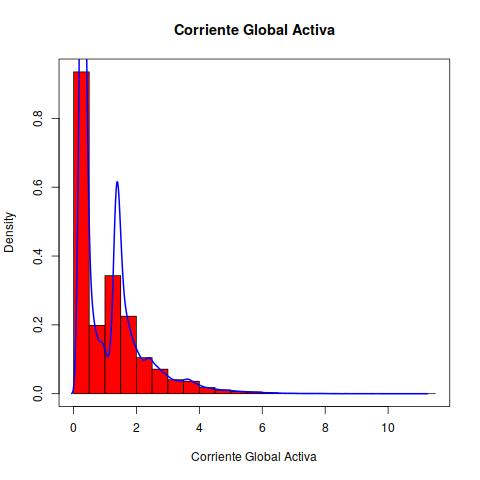
\includegraphics[width=0.45\textwidth]{img/ex1/Histograms/Histograms_GAP.jpeg} 
		\caption{Histograma de la corriente global activa}
		\label{hist:1.1}
	\end{figure}
	
	En la gráfica de cajas y bigotes se hace notar la cantidad de valores atípicos de la muestra. Se consideran atípicos los valores inferiores a $Q1–1.5*RIC$ o superiores a $Q3+1.5*RIC$, donde $Q1$ y $Q3$ son los valores del primer y el tercer cuartil y $RIC$ es el rango intercuartílico, esto es, $Q3-Q1$. En nuestro caso, hay muchos valores que se encuentran por encima de $Q3+1.5*RIC$. Los extremos de los bigotes son los últimos valores que no son atípicos, el extremo superior de nuestros datos es 3.358 y el inferior 0.076. El primer cuartil tiene el valor 0.308 y el tercer 1.528, mientras que la mediana es de 0.602. Como se puede ver en la gráfica \ref{box:1.1}, la caja está lejos de ser simétrica, lo cual corrobora la dispersión de los datos.
	
	\begin{figure}[H]
	 	\centering
	 	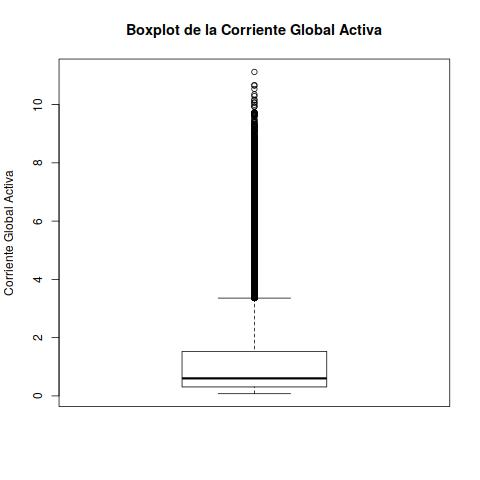
\includegraphics[width=0.45\textwidth]{img/ex1/BoxPlots/BoxPlots_GAP.jpeg} 
	 	\caption{Cajas de bisagras y bigotes de la corriente global activa}
	 	\label{box:1.1}
	\end{figure}
	
	La corriente global reactiva tiene un comportamiento similar. La media toma un valor de 0.1237145 y la mediana es 0.1, lo que significa que el 50\% de los datos posee un valor similar al promedio. La varianza y la desviación estándar toman valores de 0.0127 y 0.113 respectivamente, por lo que la gran mayoría de los datos se separan poco del promedio. Sin embargo, el coeficiente de variación es de 0.9111462, así que se puede decir que los datos son muy heterogéneos. Todo esto se puede apreciar en el histograma \ref{hist:1.2}.
	
	\begin{figure}[H]
		\centering
		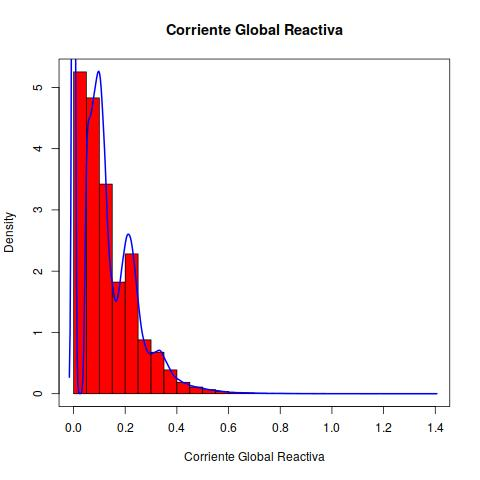
\includegraphics[width=0.45\textwidth]{img/ex1/Histograms/Histograms_GRP.jpeg} 
		\caption{Histograma de la corriente global reactiva}
		\label{hist:1.2}
	\end{figure}
	
	La gráfica de cajas y bigotes de la corriente global reactiva se comporta de manera similar a la activa con una gran cantidad de datos atípicos como se puede apreciar en la gráfica \ref{box:1.2}. El extremo inferior tiene un valor de 0.000 y el superior 0.412. El primer cuartil tiene el valor 0.048 y el tercero 0.194, mientras que la mediana es igual a 0.100.
	
	\begin{figure}[H]
	 	\centering
	 	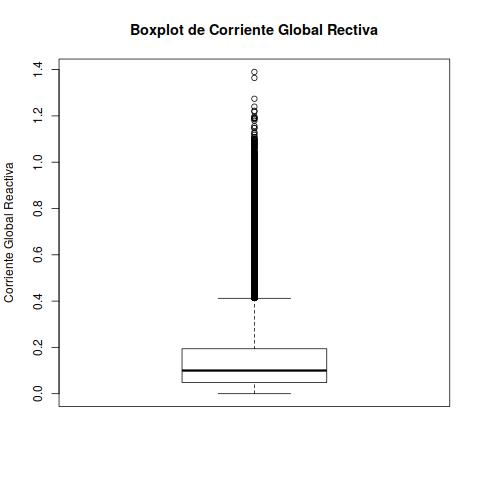
\includegraphics[width=0.45\textwidth]{img/ex1/BoxPlots/BoxPlots_GRP.jpeg} 
	 	\caption{Cajas de bisagras y bigotes de la corriente global reactiva}
	 	\label{box:1.2}
	\end{figure}
	
	En el histograma \ref{hist:1.4} se presenta una gráfica a una misma escala de la corriente global activa y reactiva, en la que se aprecia con mayor exactitud las diferencias entre estas dos muestras:
	
	\begin{figure}[H]
		\centering
		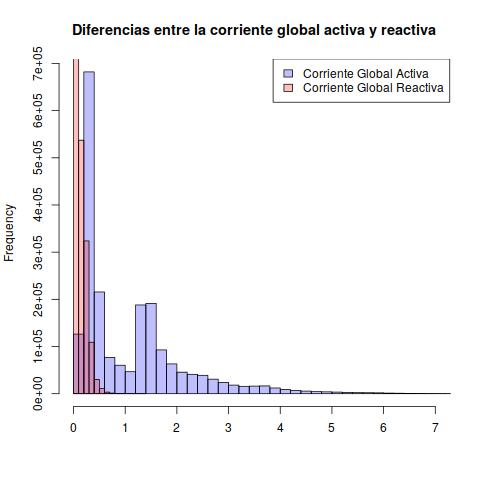
\includegraphics[width=0.45\textwidth]{img/ex1/Powers.jpeg} 
		\caption{Histograma de la intensidad global}
		\label{hist:1.4}
	\end{figure}
	
	Los datos de la muestra correspondiente a la intensidad también son muy dispersos como se aprecia en el histograma \ref{hist:1.3}. La media es de 4.627759 y dista de la mediana que tiene un valor de 2.6. La varianza y la desviación estándar son de 19.753 y 4.444 respectivamente por lo que los datos se encuentran alejados de su promedio. Además, el coeficiente de variación es del 96.04\%, por lo que los datos son muy heterogéneos.
	
	\begin{figure}[H]
		\centering
		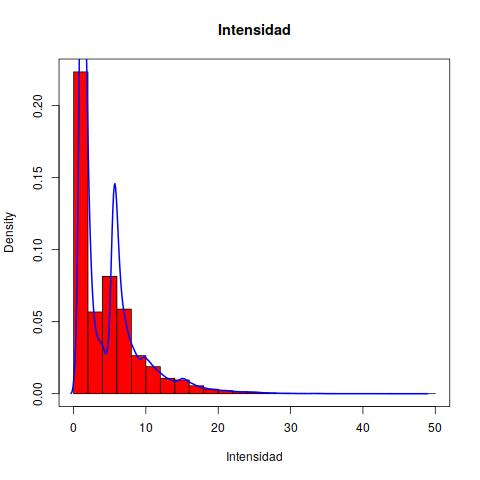
\includegraphics[width=0.45\textwidth]{img/ex1/Histograms/Histograms_Intensity} 
		\caption{Histograma de la intensidad global}
		\label{hist:1.3}
	\end{figure}
	
	La gráfica de cajas y bigotes de la intensidad también cuenta con una gran cantidad de datos dispersos. El extremo inferior de los bigotes es 0.2 y el superior 13.8, mientras que los extremos de las bisagras, que representan el primer y el tercer cuartil, tienen el valor de 1.4 y 6.4 respectivamente, y la mediana es de 2.6. Esta gráfica se puede ver en \ref{box:1.3}
	
	\begin{figure}[H]
	 	\centering
	    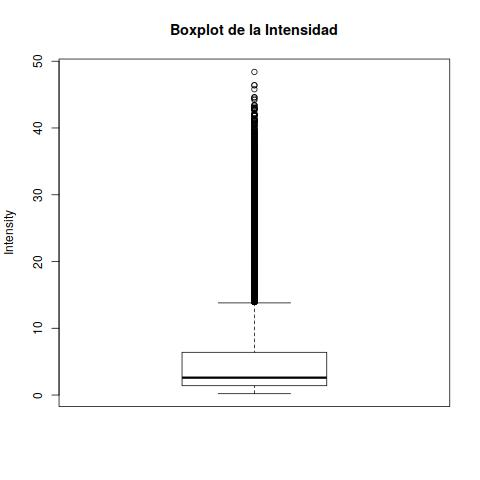
\includegraphics[width=0.45\textwidth]{img/ex1/BoxPlots/BoxPlots_Intensity.jpeg} 
	 	\caption{Cajas de bisagras y bigotes de la intensidad}
	 	\label{box:1.3}
	\end{figure}
	
%-----------------------------------------------------------------------------------
	\subsection{Muestras de Poblaciones Normales}\label{sub:ex2}
%-----------------------------------------------------------------------------------

	Se entiende por Población Estadística a la agrupación o conjunto de elementos, con características especiales, similares y comunes, que forman parte de un universo, esta condición de similitud facilita su reunión para realizar estudios estadísticos. En este problema estaremos trabajando con una población normal de tamaño 500, de donde se extraerán 8 muestras: de tamaño 20, 30, 60 y 250, 4 con reemplazo y 4 de ellas sin reemplazo.
	
	Analizando los estadísticos descriptivos en la tabla \ref{tab:2.1}, podemos observar como a medida que aumentan los datos, estos se van aproximando a una población normal. Las muestras se representan por la cantidad de elementos y se especifica si están repetidos o no, ej: 20R es la muestra de 20 elementos con repetición y 20 es la de 20 elementos sin repetición. Los estadísticos que se muestran son (en este orden) la media, mediana, varianza, desviación estándar, coeficiente de variación, lower hinge, primer cuartil, segundo cuartil, tercer cuartil y upper hinge.
	
	Se hace necesario mencionar, que a pesar de que las muestras con repetición tienen un comportamiento bastante estable en nuestro ejemplo, aproximándose a la población original, se esperaba un comportamiento diferente, ya que generalmente las muestras con repetición  entorpecen los resultados de los estadísticos descriptivos. Esto sucede porque tomar elementos repetidos puede ocasionar que no se elija una muestra verdaderamente representativa de la población con una probabilidad mayor que tomando elementos no repetidos.
	
	\begin{table*}[htb]	
		\begin{tabular}[htb]{l|lllllllll}
			Medidas  & 20R    & 20     & 30R     & 30     & 60R    & 60     & 250R    & 250    & P       \\\hline
			Media    & -0.138 & -0.326 & 0.028   & 0.255  & 0.023  & 0.069  & 0.009   & -0.036 & -0.007  \\
			Mediana  & -0.329 & -0.458 & -0.041  & 0.080  & -0.115 & 0.154  & -0.113  & -0.069 & -0.090  \\
			Varianza & 0.758  & 1.018  & 0.417   & 1.047  & 1.043  & 1.047  & 0.952   & 0.946  & 0.957   \\
			DT       & 0.871  & 1.009  & 0.646   & 1.023  & 1.021  & 1.023  & 0.976   & 0.973  & 0.978   \\
			CV       & 6.314  & 3.096  & 23.086  & 4.009  & 44.560 & 14.850 & 113.459 & 26.913 & 134.792 \\
			L        & -1.627 & -1.906 & -0.923  & -1.213 & -1.865 & -1.865 & -2.142  & -2.439 & -2.607  \\
			Q1       & -0.749 & -0.868 & -0.570  & -0.494 & -0.670 & -0.637 & -0.626  & -0.693 & -0.672  \\
			Q2       & -0.329 & -0.458 & -0.0410 & 0.080  & -0.115 & 0.154  & -0.113  & -0.069 & -0.090  \\
			Q3       & 0.569  & 0.147  & 0.524   & 0.753  & 0.512  & 0.762  & 0.640   & 0.644  & 0.649   \\
			H        & 2.126  & 2.453  & 1.581   & 3.539  & 3.240  & 2.453  & 3.240   & 2.911  & 3.539  \\
		\end{tabular}
		\label{tab:2.1}
		\caption{Estadísticos descriptivos de las muestras de la población normal}
	\end{table*}


	En casi todas las muestras la media y la mediana tienen un valor similar, lo que significa que el 50\% tiene el valor del promedio de los datos. La varianza y la desviación estándar indican poca dispersión de los datos con respecto al promedio. Tanto la media como la varianza se aproximan cada vez más a 0 y 1, que son los parámetros de la distribución normal que se genera con la población. El coeficiente de variación es muy alto en todas las muestras, lo que evidencia gran heterogeneidad. Los histogramas de las muestras y de la población se pueden ver en las gráficas siguientes, donde podemos apreciar una mayor semejanza de los datos a la gráfica de una distribución normal, a medida que estos crecen.

	\begin{figure}[H]
		\centering
		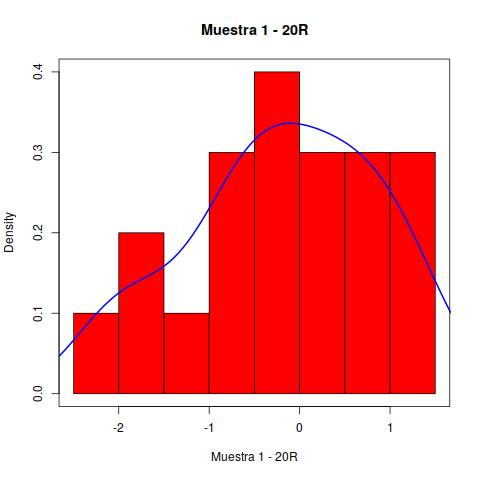
\includegraphics[width=0.45\textwidth]{img/ex2/Histograms/Histogram1.jpeg}
		% \caption{Histograma de muestras de una población normal}
		\label{hist:2.1}
	\end{figure}
	
	\begin{figure}[H]
		\centering
		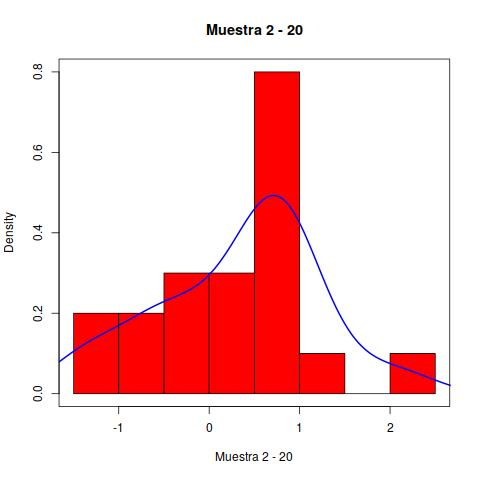
\includegraphics[width=0.45\textwidth]{img/ex2/Histograms/Histogram2.jpeg}
		\label{hist:2.2}
	\end{figure}
	
	\begin{figure}[H]
		\centering
		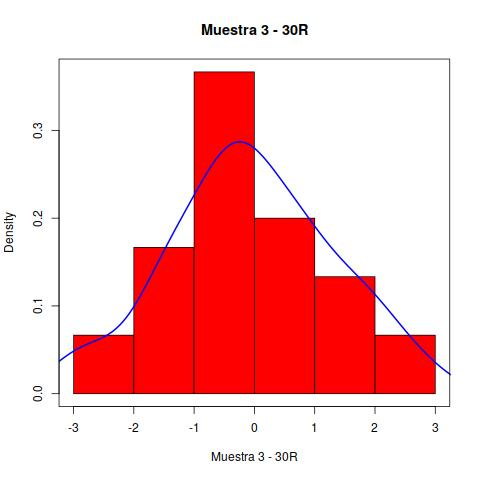
\includegraphics[width=0.45\textwidth]{img/ex2/Histograms/Histogram3.jpeg}
		\label{hist:2.3}	
	\end{figure}
	
	\begin{figure}[H]
		\centering
		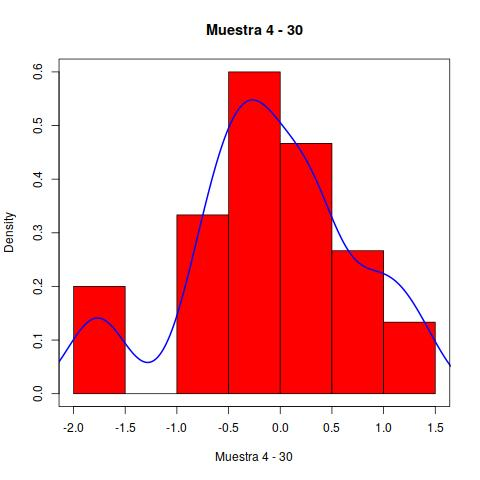
\includegraphics[width=0.45\textwidth]{img/ex2/Histograms/Histogram4.jpeg}
		\label{hist:2.4}
	\end{figure}

	\begin{figure}[H]
		\centering
		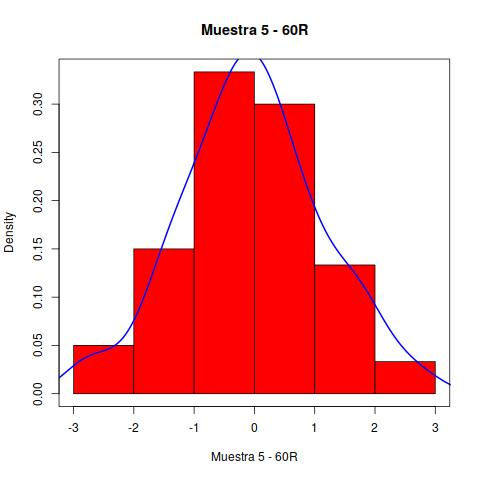
\includegraphics[width=0.45\textwidth]{img/ex2/Histograms/Histogram5.jpeg}
		\label{hist:2.5}
	\end{figure}

	\begin{figure}[H]
		\centering
		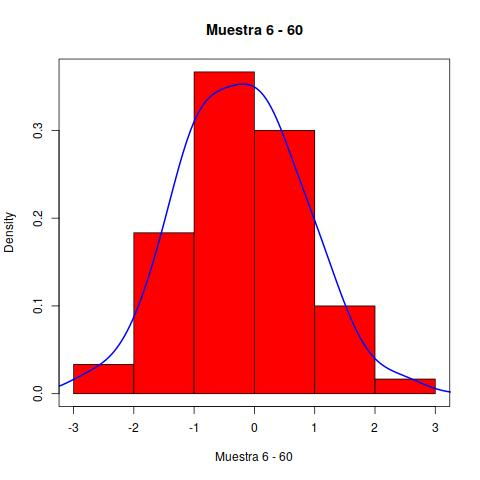
\includegraphics[width=0.45\textwidth]{img/ex2/Histograms/Histogram6.jpeg}
		\label{hist:2.6}	
	\end{figure}

	\begin{figure}[H]
		\centering
		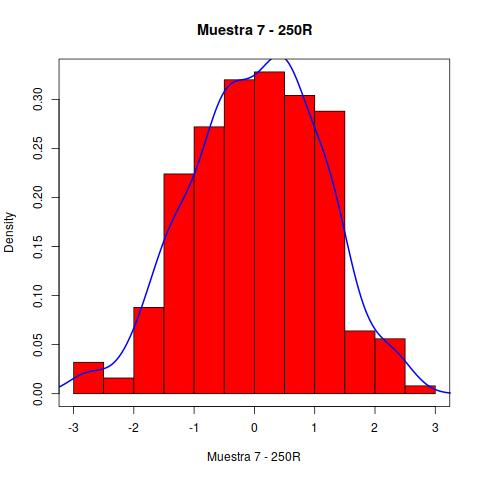
\includegraphics[width=0.45\textwidth]{img/ex2/Histograms/Histogram7.jpeg}
		\label{hist:2.7}	
	\end{figure}

	\begin{figure}[H]
		\centering
		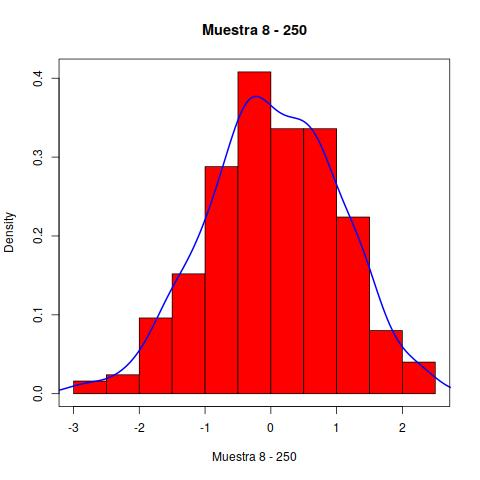
\includegraphics[width=0.45\textwidth]{img/ex2/Histograms/Histogram8.jpeg}
		\label{hist:2.8}	
	\end{figure}

	\begin{figure}[H]
		\centering
		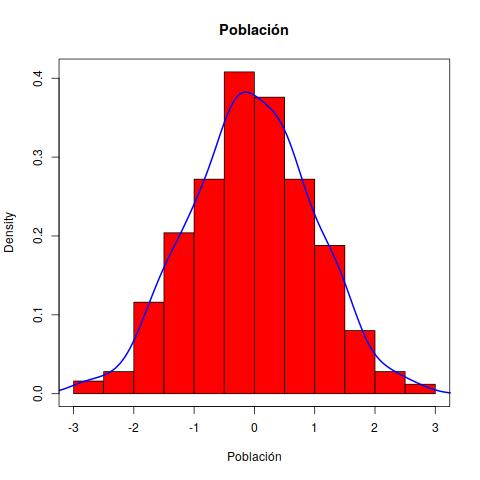
\includegraphics[width=0.45\textwidth]{img/ex2/Histograms/HistogramPop.jpeg}
		\label{hist:2.9}	
	\end{figure}
	

	Los gráficos de cajas y bigotes mostrados a continuación presentan pocos datos atípicos y tienen una forma cada vez más simétrica a medida que aumentan los datos.
	
	\begin{figure}[H]
		\centering
		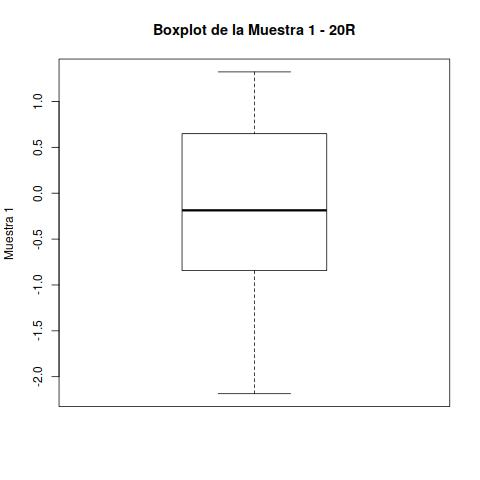
\includegraphics[width=0.45\textwidth]{img/ex2/BoxPlots/BoxPlots1.jpeg}
		\label{box:2.1}
	\end{figure}

	\begin{figure}[H]
		\centering
		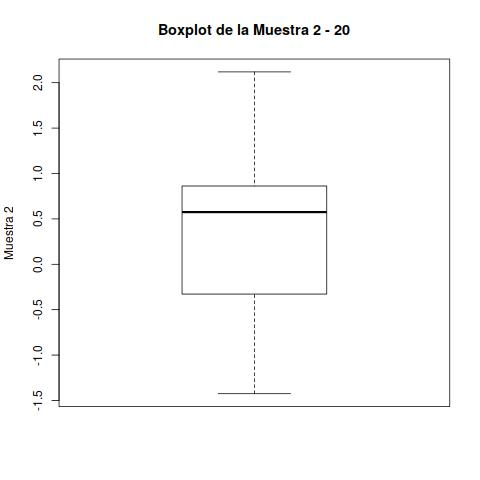
\includegraphics[width=0.45\textwidth]{img/ex2/BoxPlots/BoxPlots2.jpeg}
		\label{box:2.2}
	\end{figure}


	\begin{figure}[H]
		\centering
		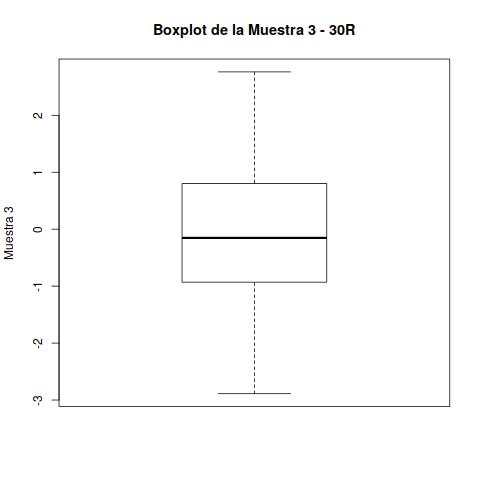
\includegraphics[width=0.45\textwidth]{img/ex2/BoxPlots/BoxPlots3.jpeg}
		\label{box:2.3}
	\end{figure}


	\begin{figure}[H]
		\centering
		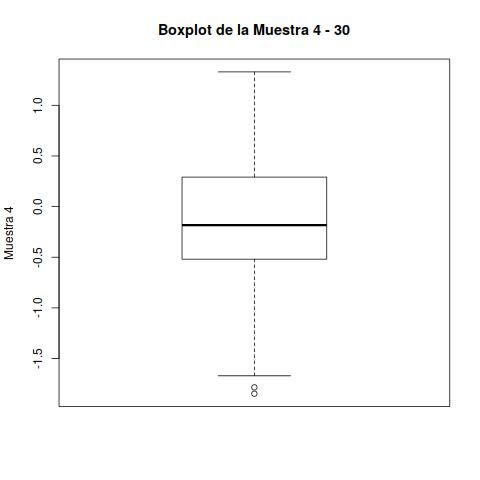
\includegraphics[width=0.45\textwidth]{img/ex2/BoxPlots/BoxPlots4.jpeg}
		\label{box:2.4}
	\end{figure}

	\begin{figure}[H]
		\centering
		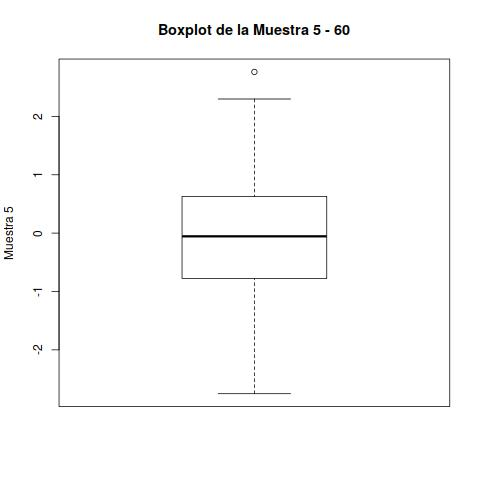
\includegraphics[width=0.45\textwidth]{img/ex2/BoxPlots/BoxPlots5.jpeg}
		\label{box:2.5}
	\end{figure}

	\begin{figure}[H]
		\centering
		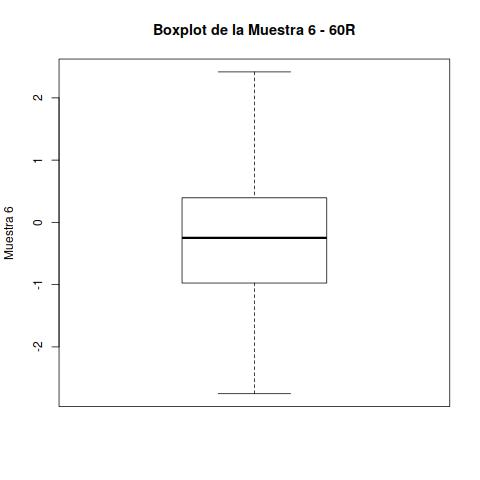
\includegraphics[width=0.45\textwidth]{img/ex2/BoxPlots/BoxPlots6.jpeg}
		\label{box:2.6}
	\end{figure}

	\begin{figure}[H]
		\centering
		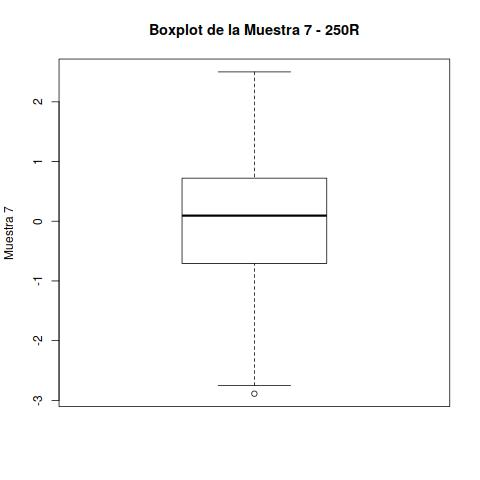
\includegraphics[width=0.45\textwidth]{img/ex2/BoxPlots/BoxPlots7.jpeg}
		\label{box:2.7}
	\end{figure}

	\begin{figure}[H]
		\centering
		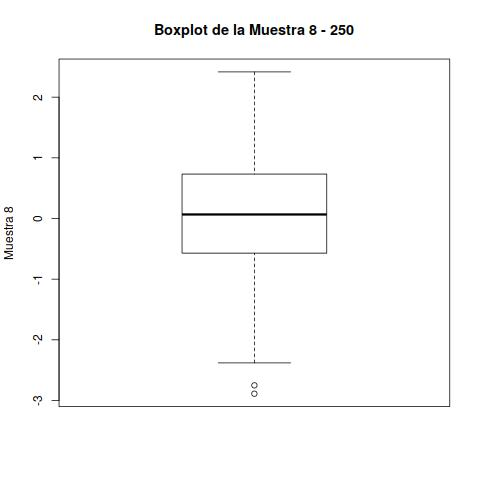
\includegraphics[width=0.45\textwidth]{img/ex2/BoxPlots/BoxPlots8.jpeg}
		\label{box:2.8}
	\end{figure}

	\begin{figure}[H]
		\centering
		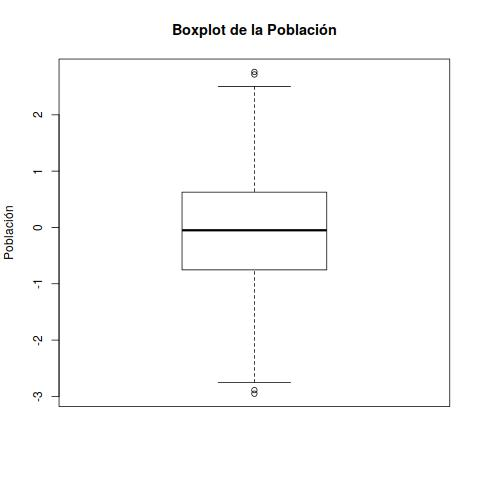
\includegraphics[width=0.45\textwidth]{img/ex2/BoxPlots/BoxPlotsPop.jpeg}
		\label{box:2.9}
	\end{figure}

	
	Los intervalos de confianza describen la variabilidad entre la medida obtenida en un estudio y la medida real de la población (el valor real). Corresponde a un rango de valores, cuya distribución es normal y en el cual se encuentra, con alta probabilidad, el valor real de una determinada variable.
	
	Con el objetivo de estimar la media, se hallan los intervalos de confianza, teniendo en cuenta dos aspectos: el conocimiento de la varianza y el tamaño de la muestra. Nuestro problema es de varianza desconocida, por lo que se considera el tamaño de la muestra. 
	
	Para $n \leq 30$ la fórmula es:
	
	\begin{equation*}
		\mu \in [\overline{X} - t_{1-\frac{\alpha}{2}}(n-1)*\frac{S}{\sqrt{n}}, \overline{X} + t_{1-\frac{\alpha}{2}}(n-1)*\frac{S}{\sqrt{n}}]
	\end{equation*}
	
	Para $n > 30$ la fórmula es:
	
	\begin{equation*}
		\mu \in [ \overline{X} - Z_{1-\frac{\alpha}{2}}*\frac{S}{\sqrt{n}}, \overline{X} + Z_{1-\frac{\alpha}{2}}*\frac{S}{\sqrt{n}}]
	\end{equation*} 
	
	Los intervalos de confianza de la media con $\alpha=0.01$ para cada una de las muestras fueron:
	
	\begin{tabular}[h]{l|ll}
		Datos & $\theta_1$ & $\theta_2$ \\ \hline
		20R   & -0.6228418 & 0.3470788  \\
		20    & -0.9771386 & 0.3253671  \\
		30R   & -0.1820719 & 0.2380432  \\
		30    & -0.2716367 & 0.7820489  \\
		60R   & -0.3238856 & 0.3697214  \\
		60    & -0.2791565 & 0.4169367  \\
		250R  & -0.1465542 & 0.1637571  \\
		250   & -0.1902655 & 0.1179829  \\
		P     & -0.1175039 & 0.1029885
	\end{tabular}
	
	El estimador de la varianza es el único que no es simétrico y que utiliza el percentil de la distribución ${\chi}^2$
	
	\begin{equation*}
		\sigma^2 \in [\frac{(n-1)*S^2}{{\chi^2}_{1-\frac{\alpha}{2}}(n-1)}; \frac{(n-1)*S^2}{{\chi^2}_{\frac{\alpha}{2}}(n-1)}]
	\end{equation*}
	
	Los intervalos de confianza para cada una de las muestras se hallaron con $\alpha=0.01$ y los resultados obtenidos fueron:
	
	\begin{tabular}[h]{l|ll}
		Datos & $\theta_1$ & $\theta_2$ \\ \hline
		20R   & 0.283004 & 1.595409 \\
		20    & 0.5103632 & 2.8771253  \\
		30R   & 0.09654249 & 0.38507383  \\
		30    & 0.607301 & 2.422309  \\
		60R   & 0.7073845 & 1.8455505  \\
		60    & 0.7124649 & 1.8588050  \\
		250R  & 0.7280407 & 1.1566233  \\
		250   & 0.7183929 & 1.1412961  \\
		P     & 0.7824524 & 1.0846381
	\end{tabular}

	Dado que la población inicial tiene una media de 0 y una varianza de 1 se puede apreciar cómo a medida que crecen los datos los intervalos de confianza acotan cada vez más dichos valores.
%-----------------------------------------------------------------------------------
	\subsection{Prueba de Hipótesis}\label{sub:ex3}
%-----------------------------------------------------------------------------------
		
		En el ejercicio se pide comparar la varianza proveniente de dos muestras diferentes, por lo que se realiza una prueba de hipótesis de dos poblaciones. Asumiendo que los datos tienen una distribución normal se usa el algoritmo de comprobación de igualdad de las varianzas de dos poblaciones normales impartido en clases. Por lo tanto, se plantean las hipótesis nula ($H_0$) y alternativa ($H_1$) siguientes: 

		\begin{table}[h]
			\centering
			$H_0: \sigma_1^2 = \sigma_2^2$ \\ 
			$H_1: \sigma_1^2 \neq \sigma_2^2$
		\end{table}

		El estadígrafo para este tipo de problema es: 
		\begin{center}
			$F = \dfrac{S_1^2}{S_2^2}$
		\end{center}

		Donde $S_1$ y $S_2$ son los estimadores de la varianza para la muestra 1 y 2 respectivamente, que en nuestro caso son la Corriente Global Reactiva y la Corriente Global Activa.

		La región crítica es el conjunto de valores de la muestra para los cuales se rechaza la hipótesis nula. Para comprobar la igualdad de las varianzas de dos poblaciones normales la región critíca es:

		\begin{center}
			$F < F_{\alpha/2}(n_1 - 1, n_2 - 1)$ o $F > F_{1-\alpha/2}(n_1 - 1, n_2 - 1)$			
		\end{center}

		Donde $n_1$ y $n_2$ son el tamaño de la muestra 1 y 2 respectivamente, $\alpha$ el nivel de significación y $F_\alpha$ es el percentil de la distribución F con $n_1 - 1$ y $n_2-1$ grados de libertad a nivel $\alpha$.

		En la prueba de la varianza el p-valor da menor que $2.2e-16$, por lo que para un valor de alfa menor que este valor no se puede decir que las varianzas sean diferentes. Para $\alpha=0.01$ se tiene que $F_{1-\alpha/2}(n_1 - 1, n_2 - 1) = 1.002531$ y el estimador es $F=87.97807$, por lo que $F > F_{1-\alpha/2}(n_1 - 1, n_2 - 1)$ y se puede rechazar la hipótesis nula. Por lo tanto, se puede decir que las varianzas son diferentes.



%===================================================================================



%===================================================================================
% Conclusiones
% %-----------------------------------------------------------------------------------
% \section{Conclusiones}\label{sec:conc}

%   En esta sección puede incluir las conclusiones de su investigación y las ideas
%   sobre la continuidad del trabajo, en el caso que aplique.

%===================================================================================

\newpage
\newpage

%-----------------------------------------------------------------------------------
%-----------------------------------------------------------------------------------

%===================================================================================
% Bibliografía
%-----------------------------------------------------------------------------------

%-----------------------------------------------------------------------------------

\label{end}

\end{document}

%===================================================================================
